\section{讲解笔记：【第14次作业笔记】 动力学(1)}
\begin{analysisbox}
本节按题目、答案和讲解笔记顺序整理。对扫描图中的结构几何关系，正文保留 OCR 可识别文字，并在图形页中保留清理后的题图，便于核对杆件、支座、荷载和尺寸。
\end{analysisbox}
\subsection*{第 1 页转写}
十一、练习题

1.基本概念

9-1设直杆的轴向变形不计，图9-63所示体系的动力自由度为（D）。（合肥工业

大学2009)

A. 1

B. 2

C. 3

D. 4

9-2

设直杆的轴向变形不计，图9-64所示体系的动力自由度为

乙。（合肥工

业大学2006)

m2

m3

图9-63

图9-64

9-3

图9-65所示结构，其动力自由度个数为

。（西安建筑科技大学2011）

9- 4

判断题。结构的自振频率、振型都反映结构本身固有的动力特性。（V）（中南

大学2009)

9 - 5

结构的振动自由度是指确定结构的

（中南大学2011)

A.全部结点位置

B.全部杆件的位置

C.全部质点的位置

D.全部动力荷载作用点的位置

9-6单自由度结构的自振频率随刚度的增大而

(增大，减小)，随质量的增

大而（增大，减小）。（北京科技大学2010)

9-7

判断题。图9－66（a）所示体系的自振频率比图9-66（b）的小。（$\times$）（西

南交通大学2009）

qm<0m

EA-=

EI

EI

12

12

12

12

(a)

(b)

图9-65

图9-66
\begin{figure}[H]\centering
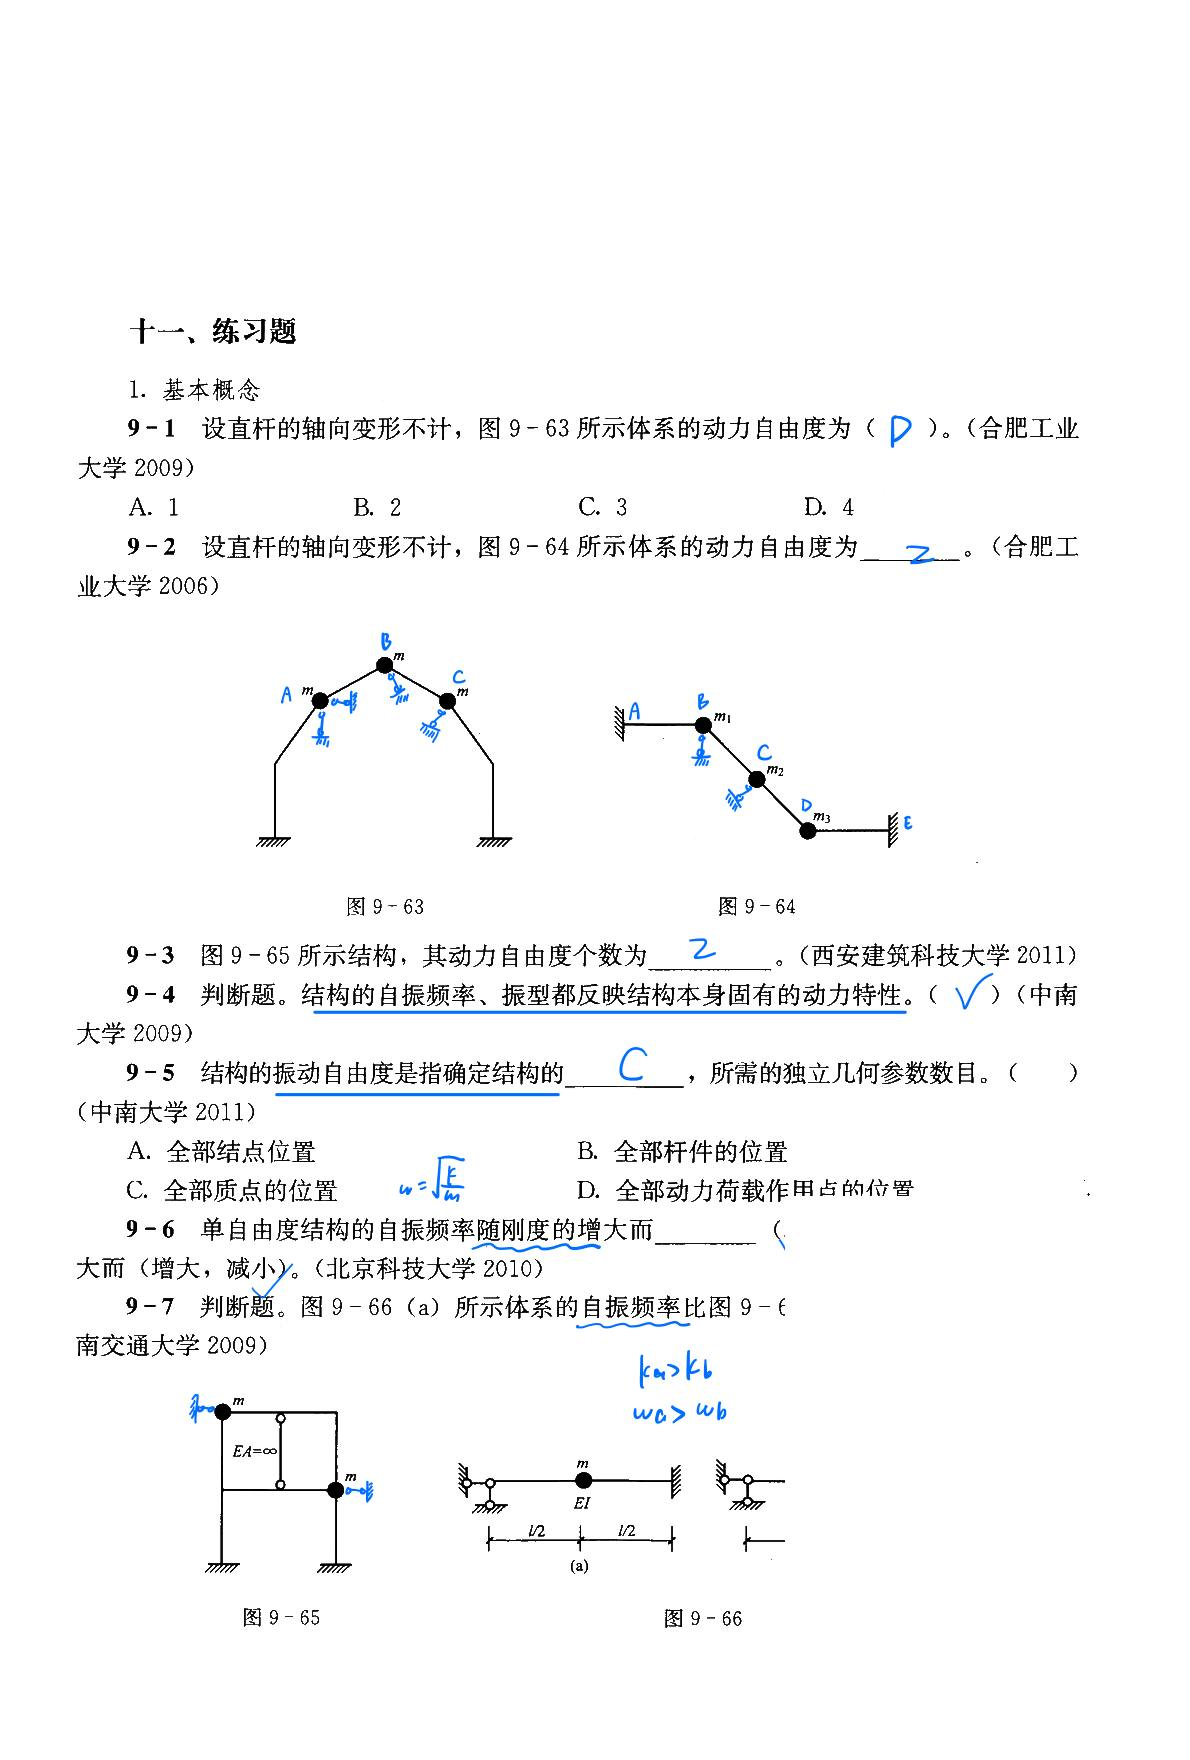
\includegraphics[width=0.92\textwidth]{figures/src33_p001.jpg}
\caption{【第14次作业笔记】 动力学(1) 第 1 页清理图形页}
\end{figure}
\subsection*{第 2 页转写}
研究生入学考试辅导丛书结构力学（第二版）

9-8判断题。对于单自由度体系，体系的内力和位移有统一的动力系数。（$\times$）（福

州大学2012)

9-9判断题。体系的动力系数一定大于1。（$\times$）（福州大学2011)

9-10使单自由度体系的阻尼增加，其结果是（

）。注：阻尼增加后仍是小阻尼

（西南交通大学2009）

WY:

B.周期不变

C.周期变短

A.周期变长

D.周期视具体体系而定

9-11

阻尼力与质点速度大小成

（正比，反比），方向相反；惯性力与质点加

速度大小成

（正比，反比），方向相反。（北京科技大学2010）

9-12

下列叙述正确的是（C）。（西安建筑科技大学2008)

X位移法是求解超静定结构的基本方法，不能用来求解静定结构

阻尼使体系的自振频率变大、使自振周期缩短

C.阻尼使体系的自振频率变小、使自振周期延长

D.力法是求解超静定结构的基本方法，也可用来求解静定结构$\times$

2.单自由度体系的计算

9-13已知图9-67中结构集中的重力G（单位为kN）位于D点，梁结构集中重力处

D点作用一简谐荷载F（t)一Fpsin(ot），其中Fp2kN，9=0.7w。EI为常数。计算梁结构

的自振频率、周期及D点处最大竖向动位移。（忽略阻尼的影响）（青岛理工大学2011）

9-14计算图9-68中结构的竖向自振频率、周期及绘制动弯矩幅值图（不计水平自

由度影响）。已知结构集中的重力G（单位为kN）位于D点，结构内B点作用一简谐荷载

F（t)=Fpsinot，其中Fp=5kN，=0.8w，EI为常数。（不计阻尼的影响）（青岛理工大学

2012)

Fp()

IFp()

2EI

3m

2m

2m

图9-67

图9-68
\begin{figure}[H]\centering
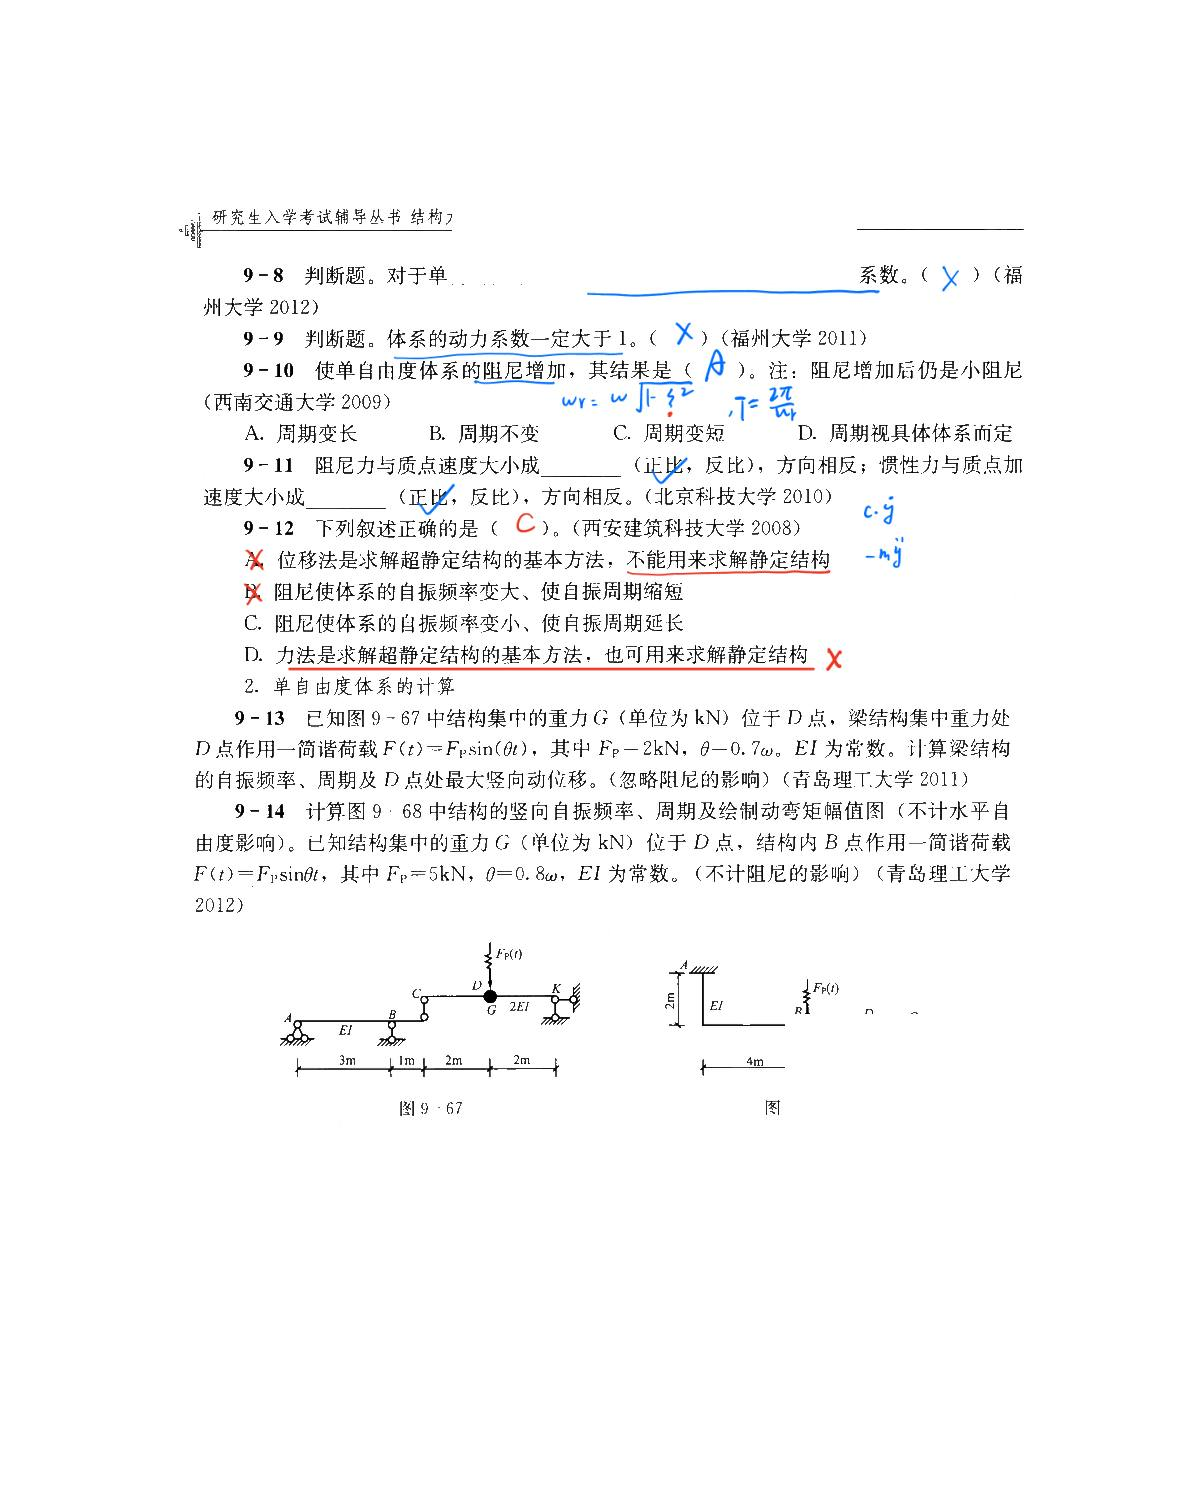
\includegraphics[width=0.92\textwidth]{figures/src33_p002.jpg}
\caption{【第14次作业笔记】 动力学(1) 第 2 页清理图形页}
\end{figure}
\subsection*{第 3 页转写}
O

nnnn

二

一

一

i

hhhdi

913

n

8 2言

2 1 1

x1主生3

i 3论式分言言

w 15 5

T瓷

2不答冽磊

yst言2

$\beta$ 磨

二115 Ya 毙n

9 14

2

12

年1 4

N d

i

8  lix2 1 1 六十 x4 2 25

2 2 2 二毙2

w 5m nai

Fu

2不器

一

jmyi

Alinot

Yltt Aocosot

可 鼠琞只售4Fp.it22 4Fp  

二器

A $\beta$yst 忐

2

毙

二毙i

747

d

mA0三mx 器2 0.5 3Um 二步

4Fl

4Fi

Mp
\begin{figure}[H]\centering
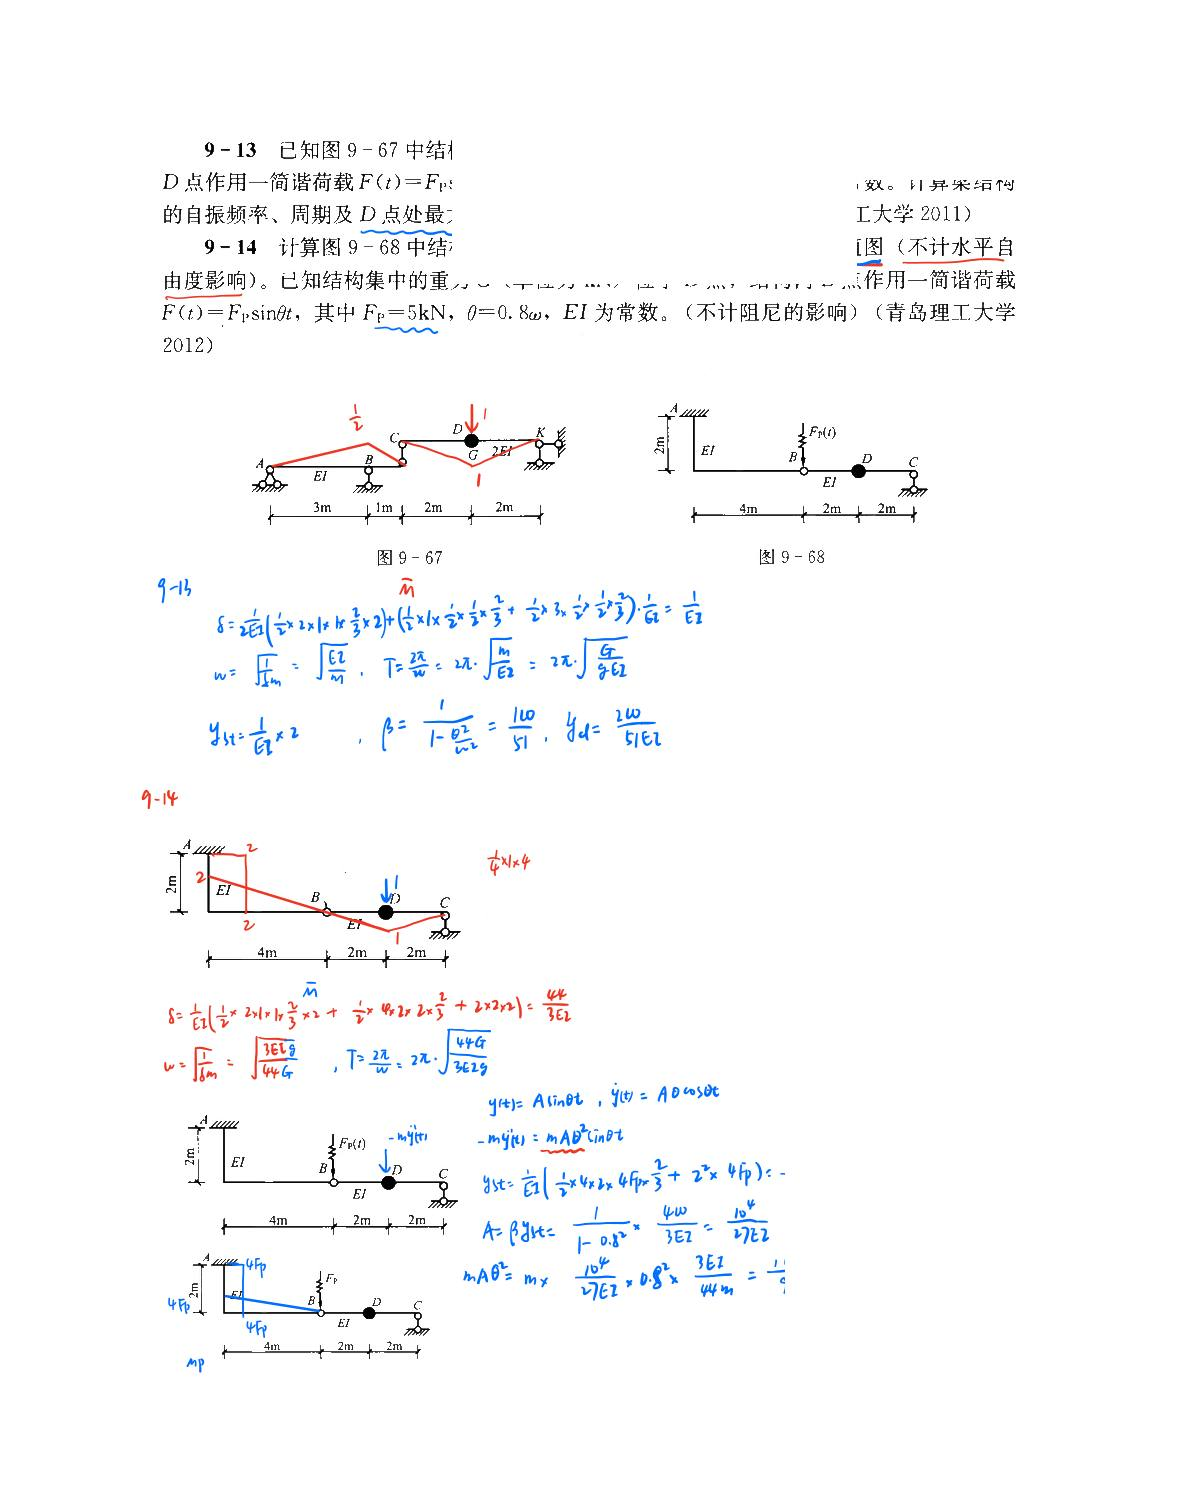
\includegraphics[width=0.92\textwidth]{figures/src33_p003.jpg}
\caption{【第14次作业笔记】 动力学(1) 第 3 页清理图形页}
\end{figure}
\subsection*{第 4 页转写}
6.16

4m

2m + 2m

9-15已知图9-69中m=3t，Fp=8kN，干扰力转速为150r/min，不计杆件质量，

EI=6X103kN m ，求质点的最大位移。（天津大学2011）

9-16试求图9-70所示体系稳态阶段的最大弯矩。0=0.5w（为自振频率），不计

阻尼。（西南交通大学2012）

Fpsingt

EI

2m

2m

图9-69

图9-70

m= 3000 k5

EI

EI

2m

Fpt'

8knx 2 m3

dits

bx bx (o?kw.mz

: 3873

150$\times$2元

509

$\beta$= 1

m (a1 *1'7 =d -h =pb
\begin{figure}[H]\centering
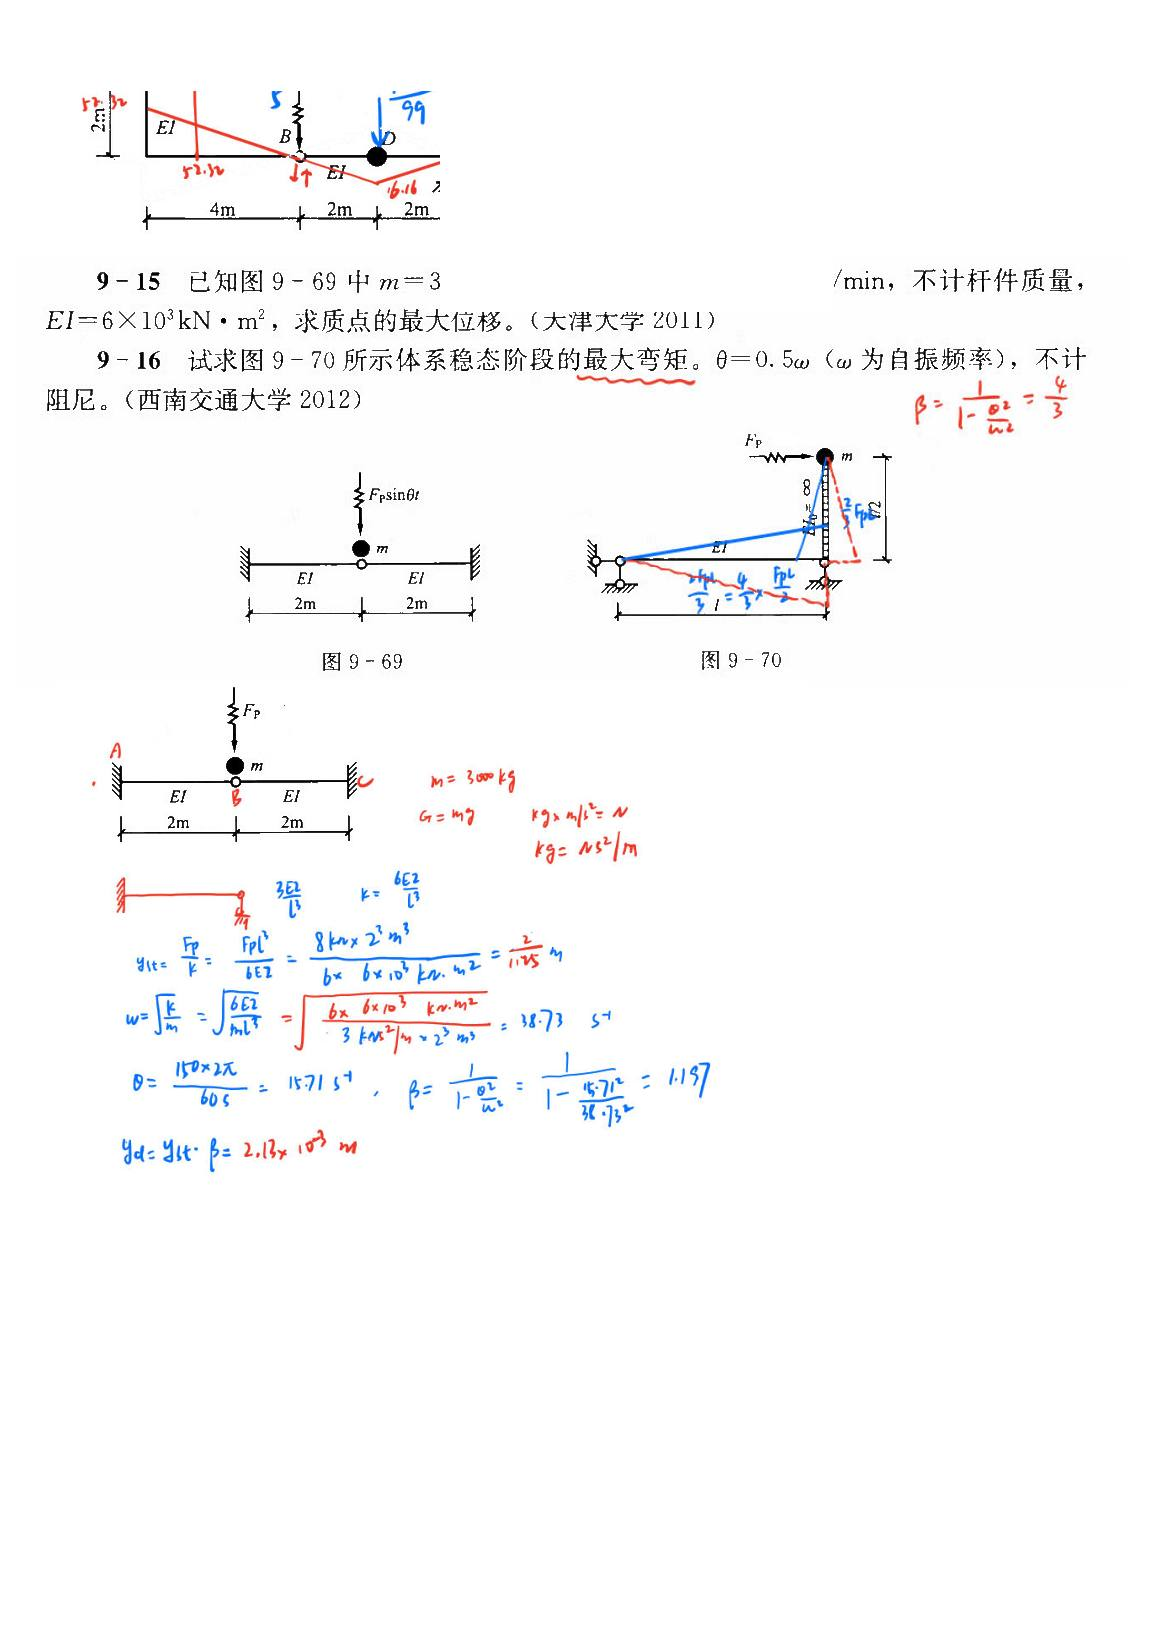
\includegraphics[width=0.92\textwidth]{figures/src33_p004.jpg}
\caption{【第14次作业笔记】 动力学(1) 第 4 页清理图形页}
\end{figure}
\subsection*{第 5 页转写}
9-17图9-71所示结构承受简谐荷载Fpsinot的作用，设各柱EI相同，不计柱的质

5EI

量，不计阻尼。试求质量 的最大动位移。设一

（湖南大学2012)

mh3

9-18图9-72所示结构承受Fpsinot简谐荷载的作用。各杆EI相同，不计杆的质量

和轴向变形，不计阻尼。设

w，为结构的自振频率。试求：（1）体系的振动微分方

程：（2）质点m的振幅A。（重庆大学2009)

Fpsingt

BEL

图9-71

图9-72
\begin{figure}[H]\centering
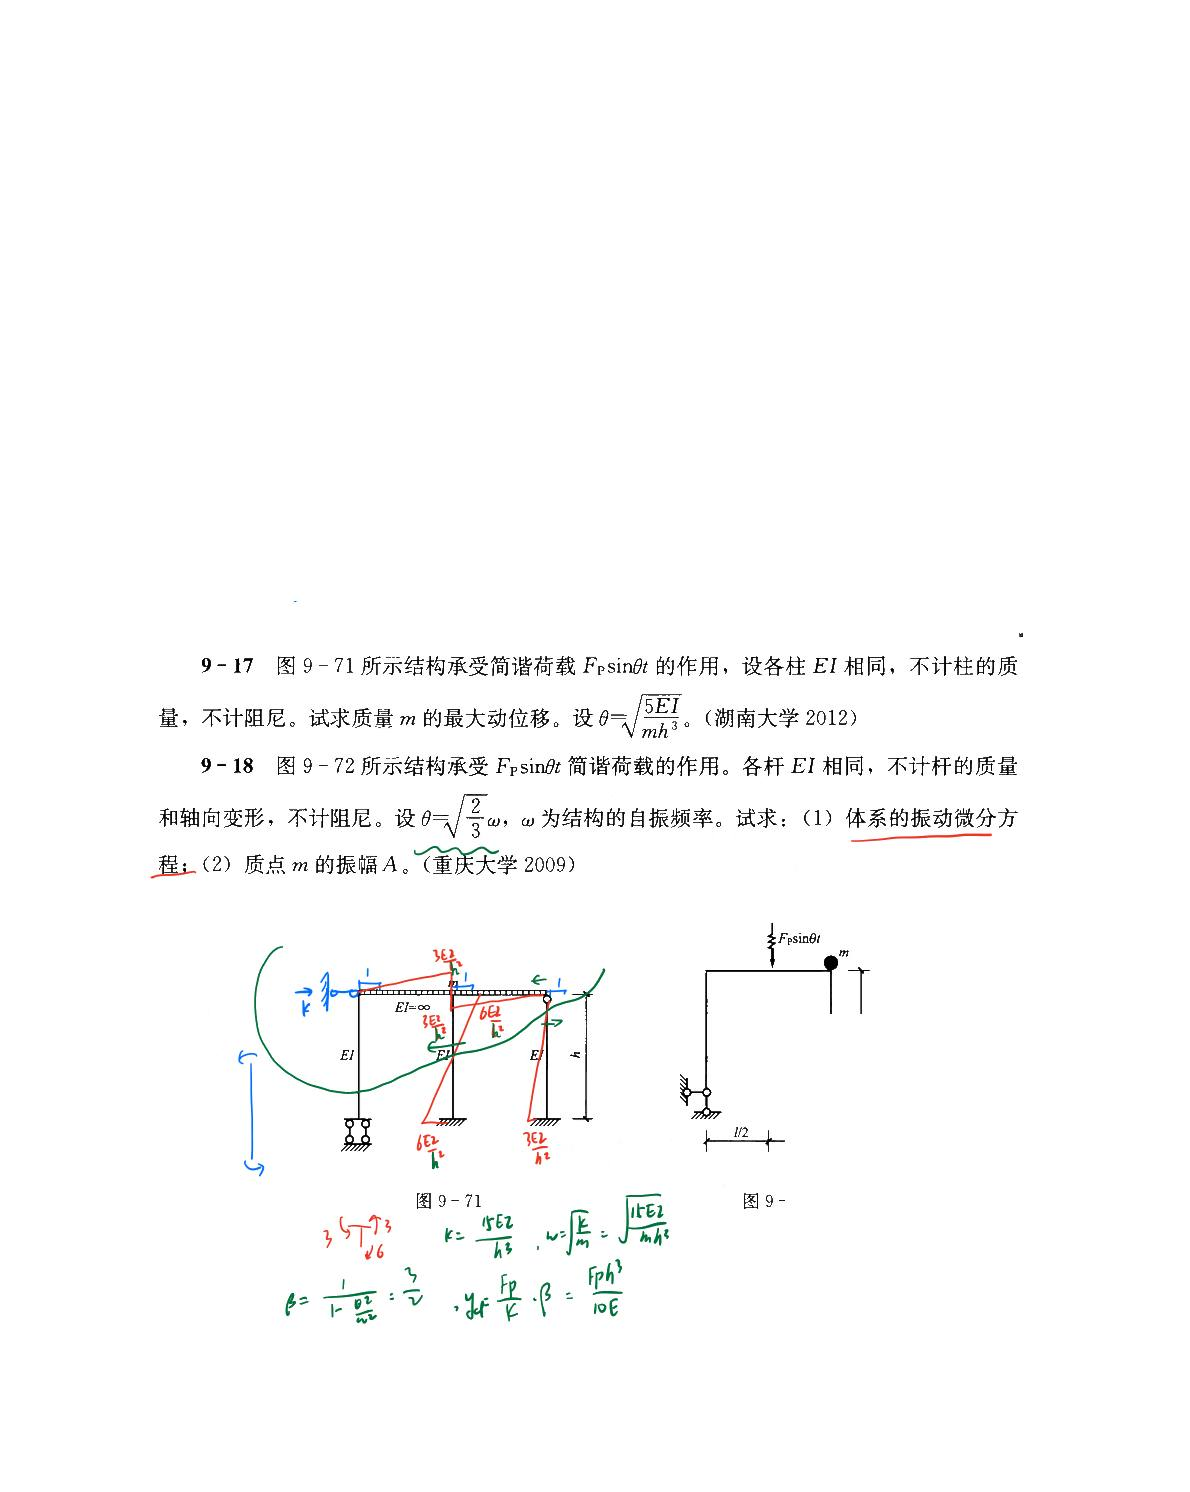
\includegraphics[width=0.92\textwidth]{figures/src33_p005.jpg}
\caption{【第14次作业笔记】 动力学(1) 第 5 页清理图形页}
\end{figure}
\subsection*{第 6 页转写}
myit

I

ylt

fnl myit.lt onpsinot

2器工jiitylt

二鼠工sinot

$\beta$

二熊

二3

yd $\beta$yst

3器

sn 垚 xlxix2 器

oip  zlixlxi x

器

1

1 dhmg

Fp i

古

MI

MP
\begin{figure}[H]\centering
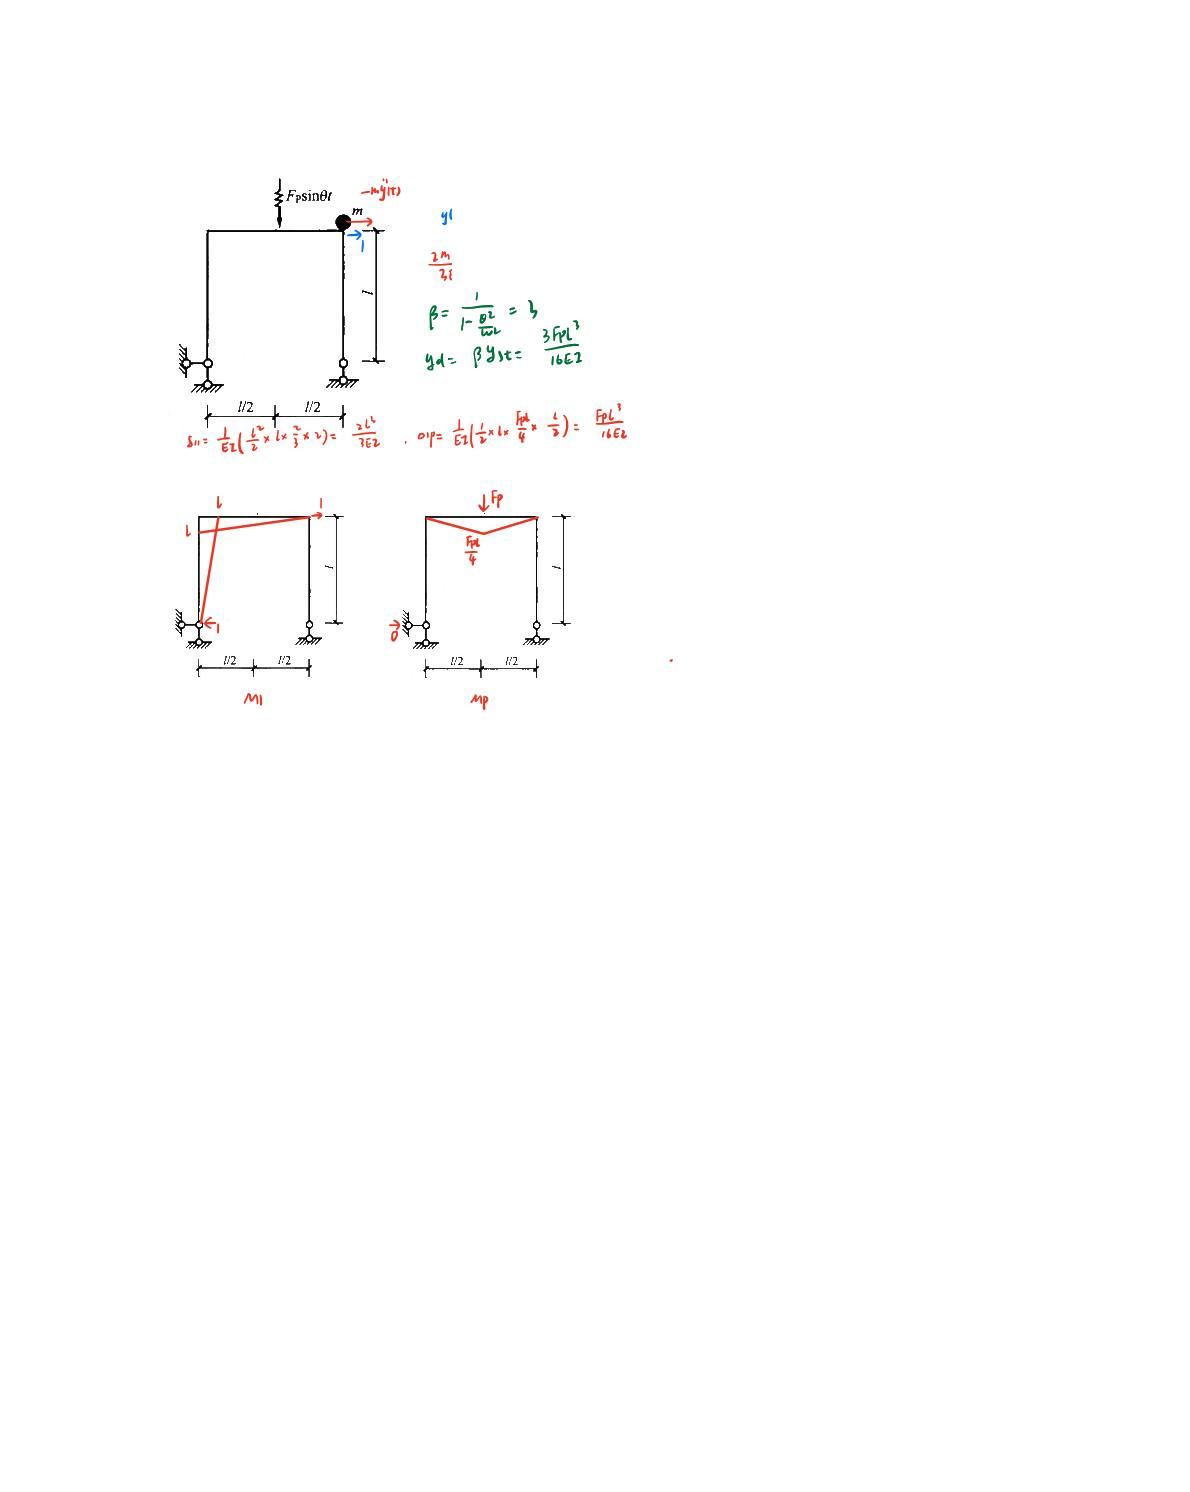
\includegraphics[width=0.92\textwidth]{figures/src33_p006.jpg}
\caption{【第14次作业笔记】 动力学(1) 第 6 页清理图形页}
\end{figure}
\subsection*{第 7 页转写}
TT

5 u  

1 5in

出

nb.it

上

1

919

m

igmmmnn

snm

t.sn

me

1 Sum

fum.tn

0 Ii S1i

喜1 x33 33

二昆

州

su二言123 2 二瓷

d

I2

sinfu

言1 x2

一是2

1

1

誓

一入

一管

m L

m

石

一管

管nl

入1

39.2483筐

入2 2.757管

u

0.16层

ur

0.603唇

8
\begin{figure}[H]\centering
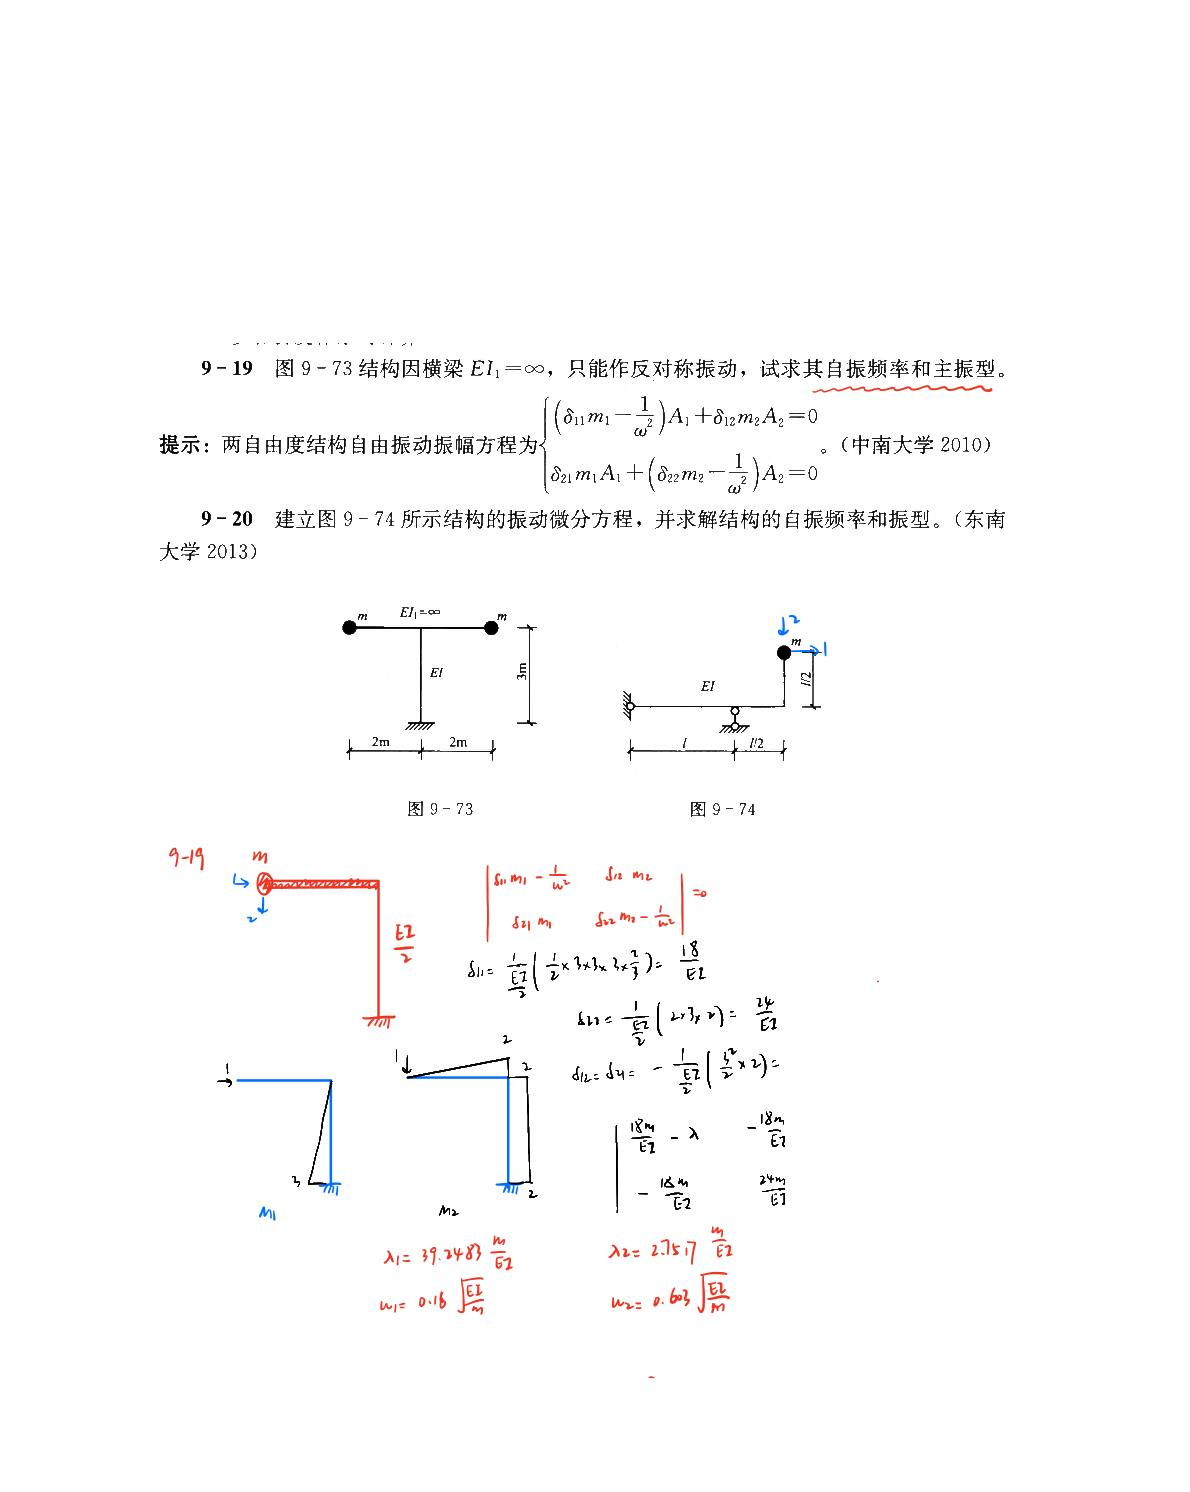
\includegraphics[width=0.92\textwidth]{figures/src33_p007.jpg}
\caption{【第14次作业笔记】 动力学(1) 第 7 页清理图形页}
\end{figure}
\subsection*{第 8 页转写}
然

二一器w

以

名

喜gnm t

二型

器

s器六

\_2757

器急

华

了心In

 nii

yit Siil myitnltticl.myit

yzti.sul

myiltlltsuzl.myit

d

l

n d

i

i

 

 

MI

811言1出ixix   t xix it  xlxix望3

二品

512二521二垚 xlx  xix it 出 x ix

二t 

822 言 xixix诊十 xlxixix

二箍

器

一入

器

1 器

1

wi

171昏

了

入1 0.3461呈1

入2 0.01883 瓷

wn589區恶i

哔

on

一哔

9-20
\begin{figure}[H]\centering
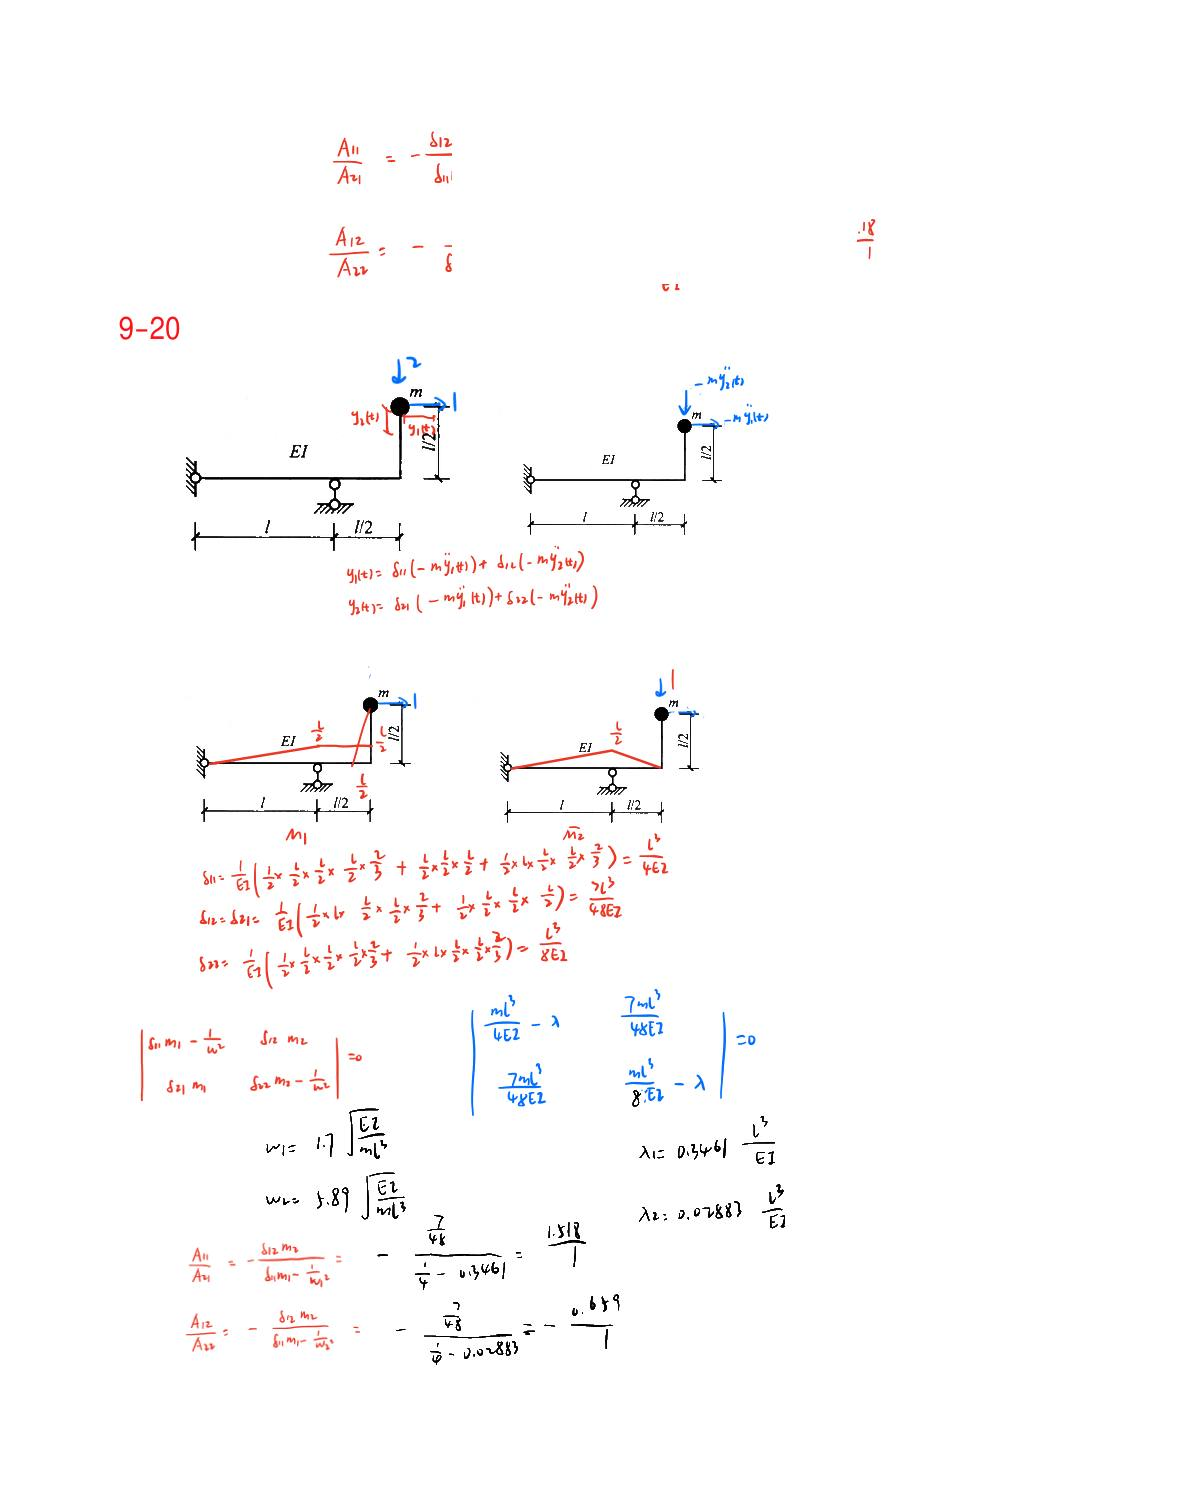
\includegraphics[width=0.92\textwidth]{figures/src33_p008.jpg}
\caption{【第14次作业笔记】 动力学(1) 第 8 页清理图形页}
\end{figure}
\subsection*{第 9 页转写}
4.对称性的利用

9-21求图9-75所示体系的自振频率和主振型，EI=常数。（河北工业大学2012

西南交通大学2008）

9 -22

试求图9-76所示对称体系的最低自振频率。EI=常数。（西南交通大学20

重庆大学2009类似）

14:25
\begin{figure}[H]\centering
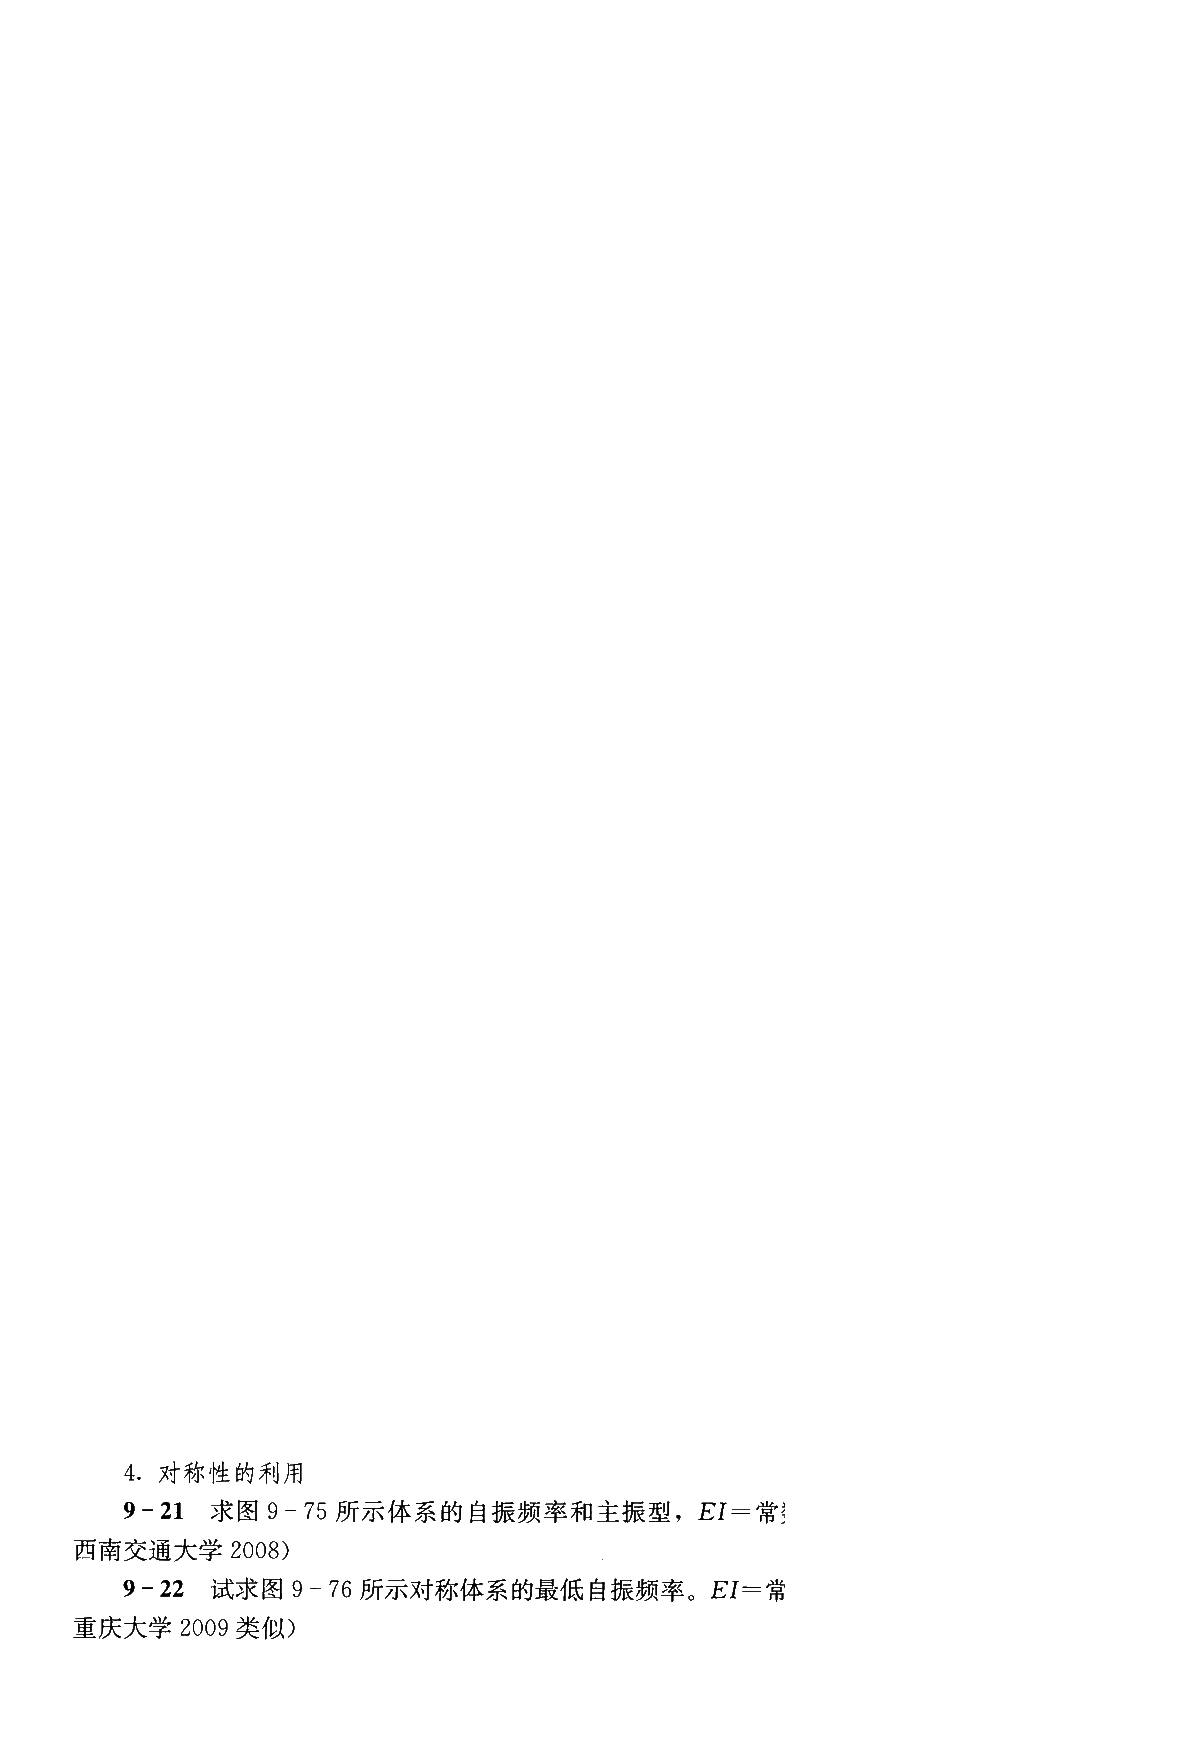
\includegraphics[width=0.92\textwidth]{figures/src33_p009.jpg}
\caption{【第14次作业笔记】 动力学(1) 第 9 页清理图形页}
\end{figure}
\subsection*{第 10 页转写}
n

n

i

i

o39

m

nlmnzyinii.in

1跈

1

i 

M

A

和

M分

mp

9I

t

s 言lixaxv3axaxi ixax0laxax引

言lixzaxo

3axaxi.ge器

wjj 

赢

一

1器

we

19

和蒸

n

器卡

29

29

嘉

 

8垚ixaxzaxzax3十 x29 29 29 3 二管

w jtit

Wi

器

二合

1 n

9 22

D
\begin{figure}[H]\centering
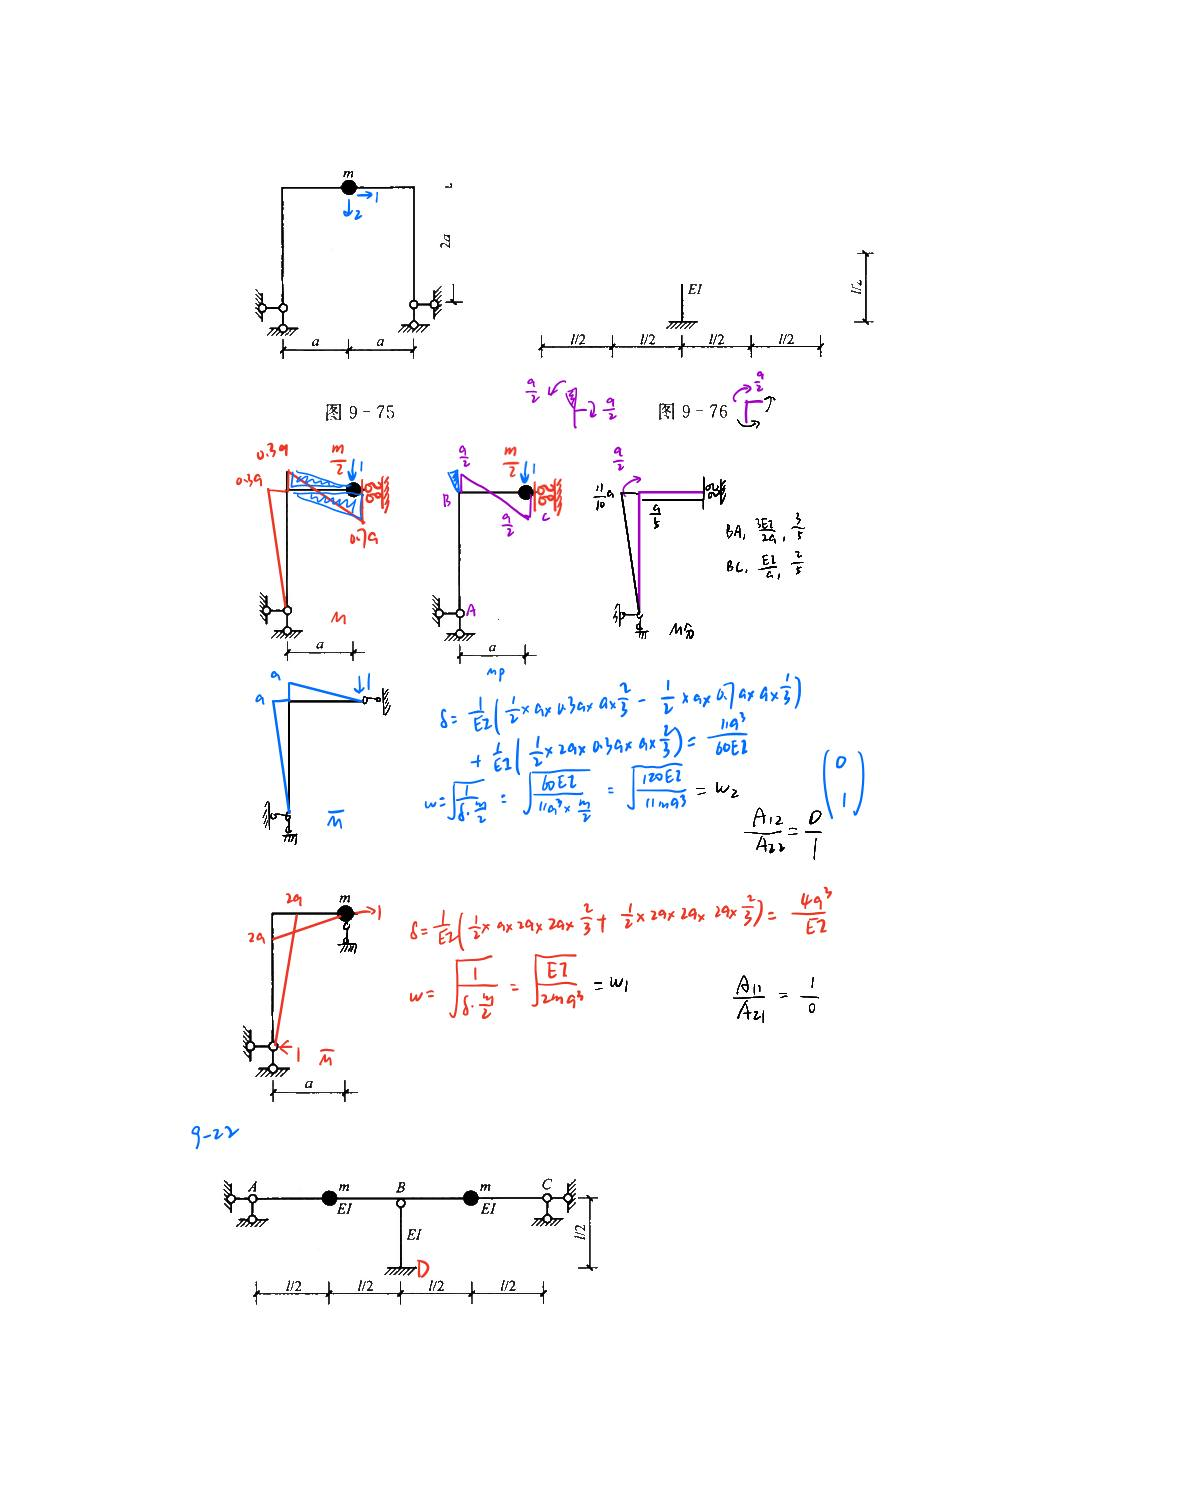
\includegraphics[width=0.92\textwidth]{figures/src33_p010.jpg}
\caption{【第14次作业笔记】 动力学(1) 第 10 页清理图形页}
\end{figure}
\subsection*{第 11 页转写}
在

5言lixix x x 

二彘

山

wt 

心



嘉
\begin{figure}[H]\centering
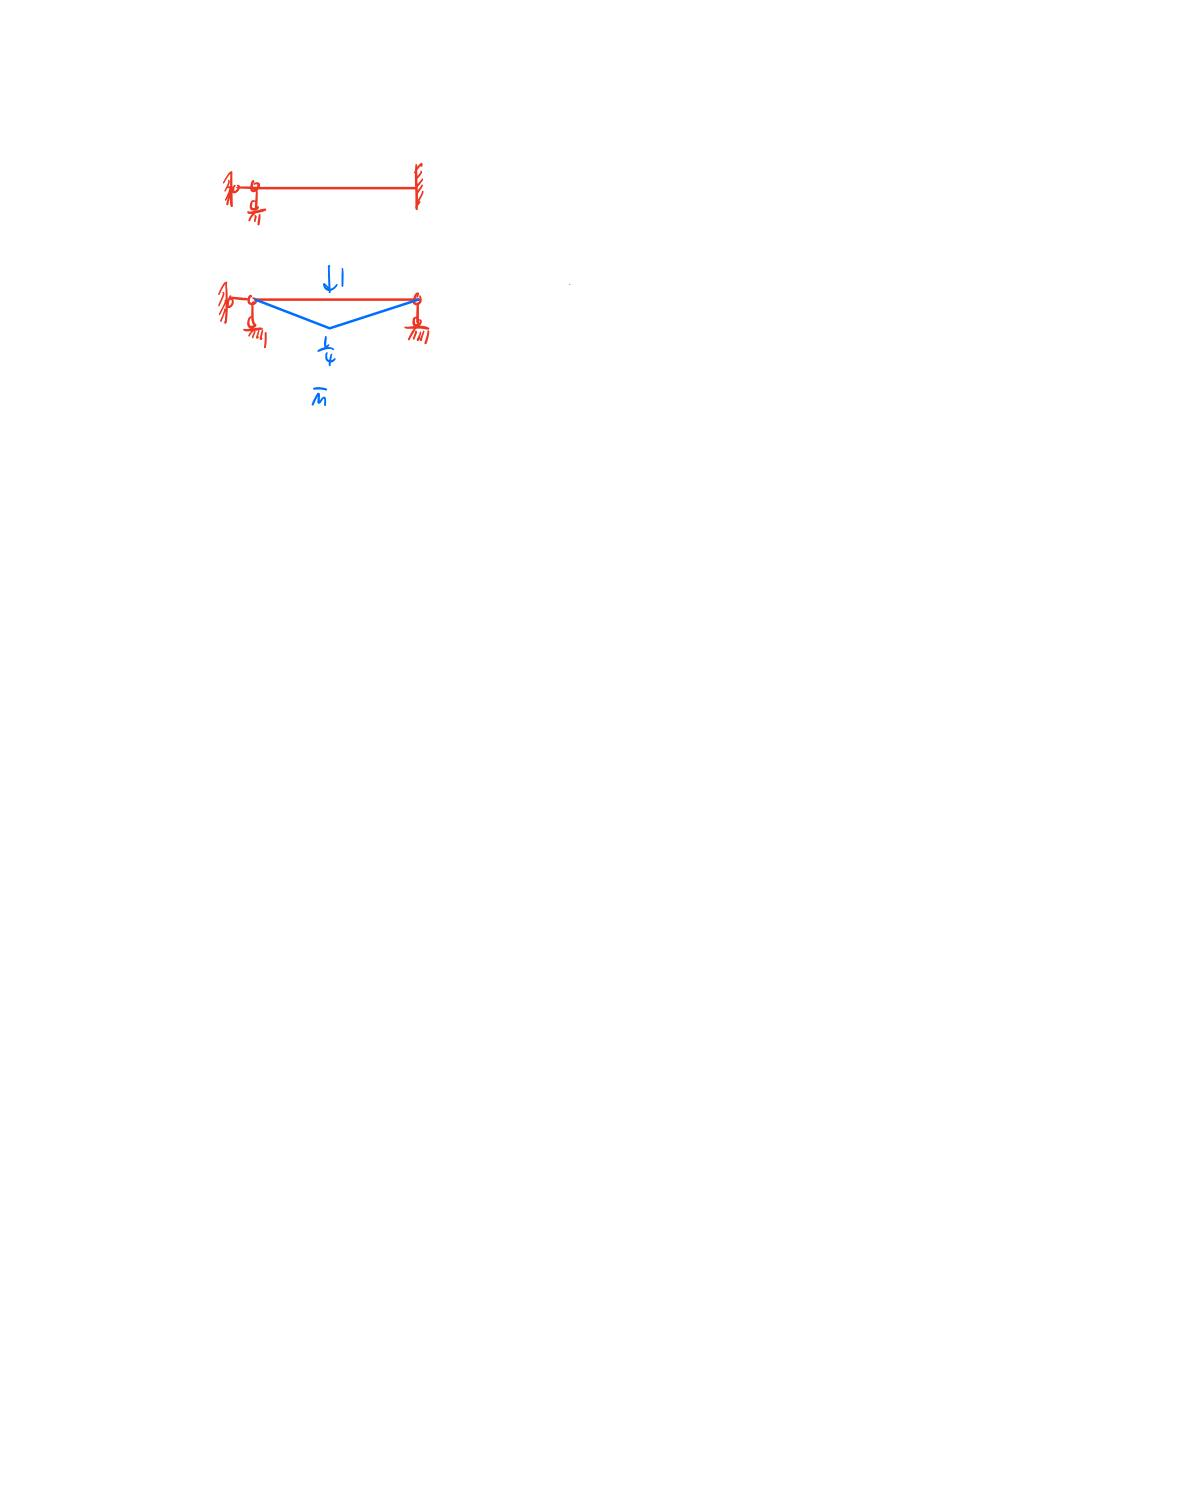
\includegraphics[width=0.92\textwidth]{figures/src33_p011.jpg}
\caption{【第14次作业笔记】 动力学(1) 第 11 页清理图形页}
\end{figure}
\subsection*{第 12 页转写}
研究生入学考试辅导丛书结构力学（第二版）

EI

EI

图9-75

图9-76

5.弹簧（支座）的计算

24EI

9-23图9-77（a）所示单跨梁的自振频率为=

今在其集中质量m处加一

5ml3

竖向弹簧支承，如图9-77（b）所示，设弹簧的刚度系数为k，则图9－77（b）的自振频率

（北京科技大学2009）

EI

Fml?

24El

315

(a)

(b)

图9-77

9 - 24

求图9-78所示体系的自振频率。质量为m，各杆EI=常数，弹性支承的刚度

系数k=EI/13。（湖南大学2010)

9 -25

求图9－79所示结构的自振频率。（福州大学2008)

EI=00

图9-79

9-26试求图9-80所示体系的自振频率及质量m的最大动力位移，设6=0.5，

弹簧刚度k0.5EI/13，各杆的EI值相同，计算时不考虑阻尼影响。（清华大学2009）

Fp!

图9-80

426
\begin{figure}[H]\centering
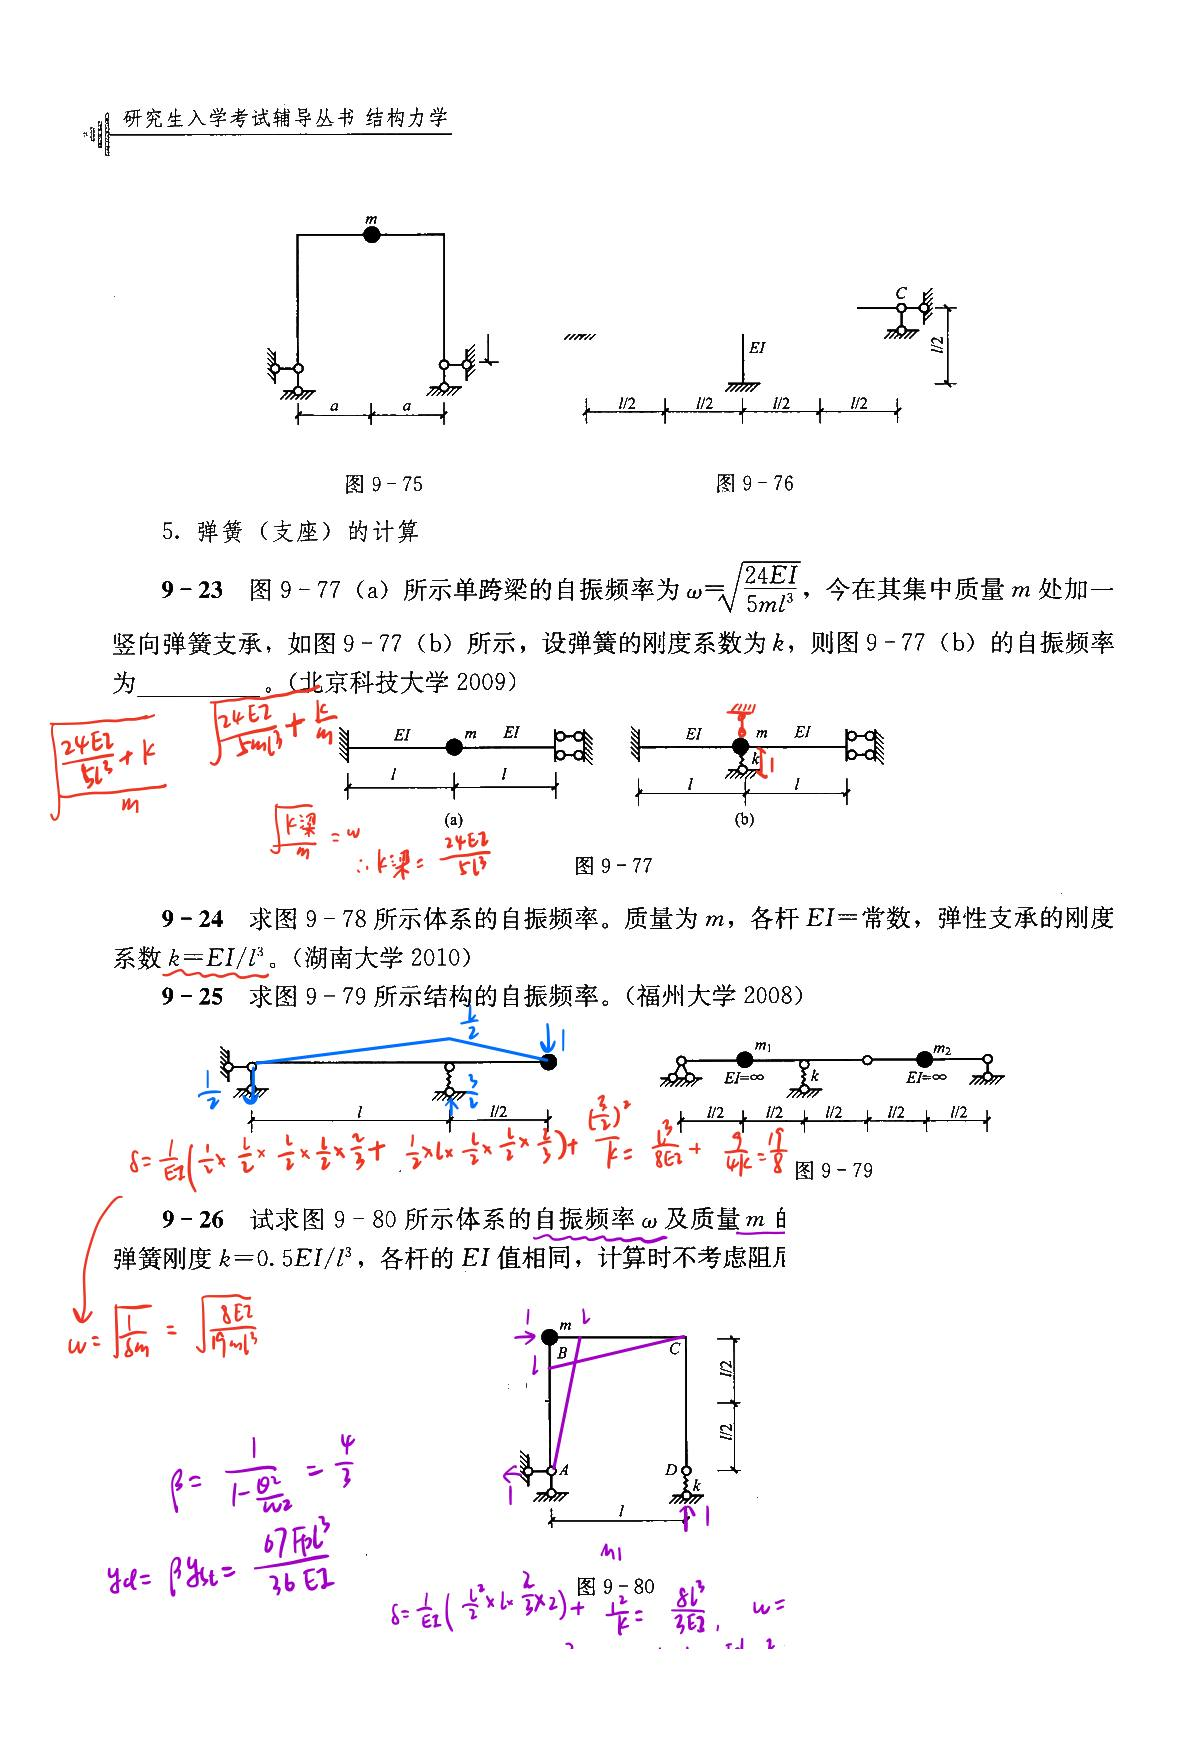
\includegraphics[width=0.92\textwidth]{figures/src33_p012.jpg}
\caption{【第14次作业笔记】 动力学(1) 第 12 页清理图形页}
\end{figure}
\subsection*{第 13 页转写}
925

C

D

ii

I

I

品

i

i

然以

小品5miit

m it xit

2kyltlxttl.fmiyt 北一0.75miyitx2540

o5m y'It 十imzyitit 2kg1十1 0

4mi 9mnyit

16kylt 0

yt t 器

1gniylt

0

it t w yIt

0

i w
\begin{figure}[H]\centering
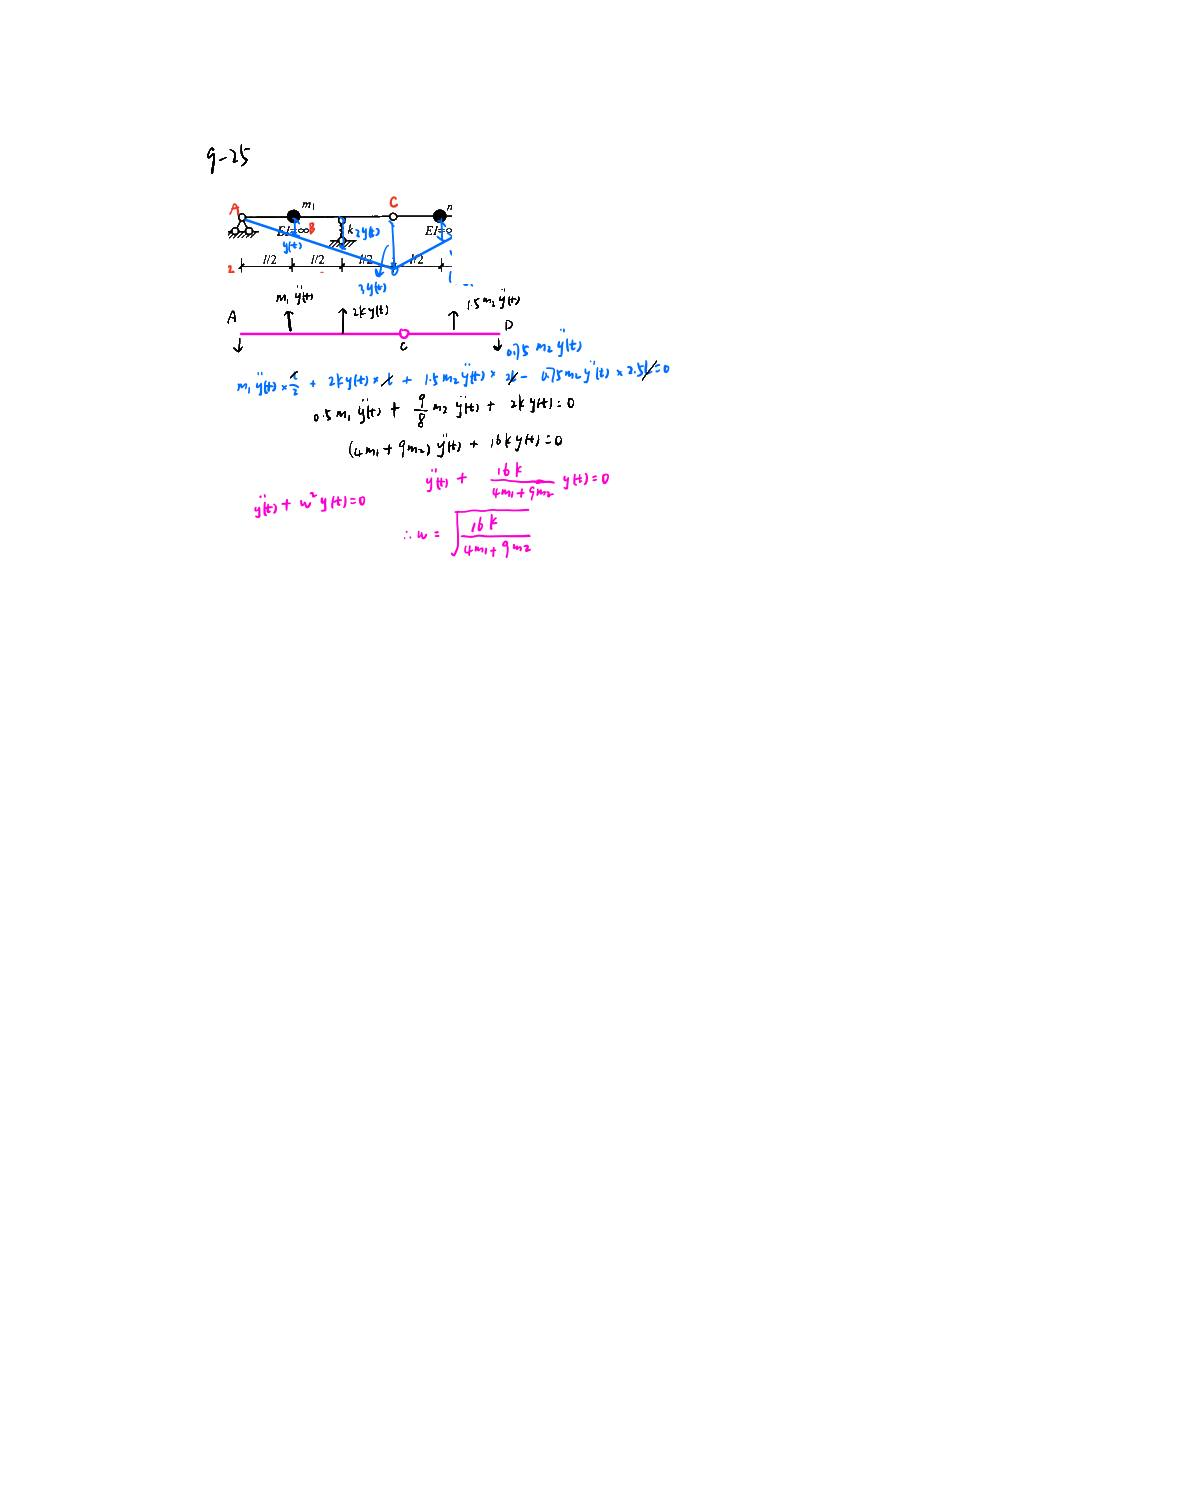
\includegraphics[width=0.92\textwidth]{figures/src33_p013.jpg}
\caption{【第14次作业笔记】 动力学(1) 第 13 页清理图形页}
\end{figure}
